\section{Results}

The results returned by the optimization algorithm are shown in \ref{fig:badPlot}. We observe that the flight path nicely avoids the clouds in the center, while at the same time the plane flies into the sunny area, to charge its batteries. In addition the path starts at the start point and ends at the endpoint. A condition we fed into the solver initially. 
At this point it is important to note, that the plots are not plotted as functions of time but as functions relative to the position in the path vector. When taking a closer look at the speed and sun gain plots we observe, that the plane speeds up initially and slows down when it reaches the sunny region that is close to it's destination. A behavior that we would expect from a good solver, since it leads to higher battery levels if the plane spends more time in the sunny regions.

\begin{figure}[width=15cm]
\begin{minipage}[c][11cm][t]{0.5\textwidth}
  \vspace*{\fill}
  \centering
  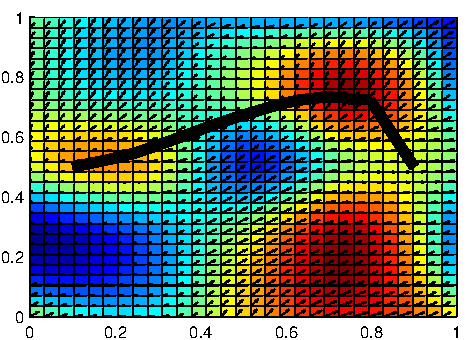
\includegraphics[width=10cm,height=10cm]{../src/plot/fancy/path}
  \subcaption{test figure one}
  \label{fig:test1}
\end{minipage}%
\begin{minipage}[c][11cm][t]{.5\textwidth}
  \vspace*{\fill}
  \centering
  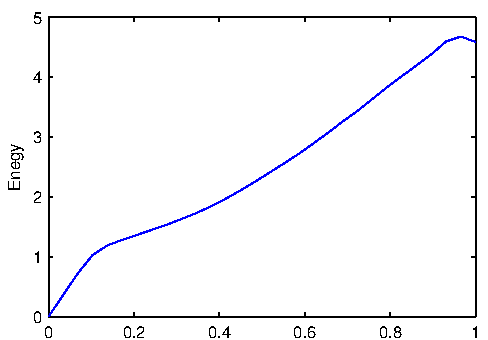
\includegraphics[width=4.5cm,height=4.5cm]{../src/plot/fancy/Energy}
  \subcaption{test figure two}
  \label{fig:test2}\par\vfill
  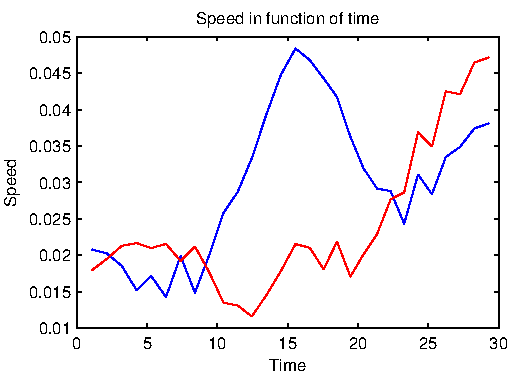
\includegraphics[width=4.5cm,height=4.5cm]{../src/plot/fancy/speed}
  \subcaption{test figure three}
  \label{fig:test3}
\end{minipage}
\caption{The left plot shows the optimized path for our optimization problem. The speed of the airplane (blue) and the relative speed (red) are shown in the bottom right position. In top the right position we show the amount of energy that's converted in the plane's solar cells as a function of time. The bottom left shows the acceleration as a function of time. The bottom middle plot depicts the energy level in the battery throughout the flight. Finally the bottom right plot depicts the derivative of the cost function.}
\label{fig:badPlot}
\end{figure}

